\chapter{Antecedentes}
\label{ch:antecedentes}

En este capítulo se presentan los antecedentes que fundamentan el sistema propuesto. En primer lugar, el marco teórico define los conceptos del dominio y las técnicas sobre las que se apoya el trabajo. A continuación, el estado del arte revisa los enfoques de detección publicados, ubica la propuesta frente a las soluciones disponibles en el mercado mediante el análisis de competencia y cierra con los hallazgos que delimitan la oportunidad del trabajo.

\section{Marco teórico}

En esta sección se definen los conceptos sobre los que se apoya el resto del trabajo. En primer lugar se delimita el fenómeno de la desinformación y su taxonomía. A continuación se presentan las técnicas de NLP, desde las representaciones clásicas hasta los modelos generativos, la búsqueda vectorial, el esquema general de la detección automática, con la recuperación de evidencia y la detección de postura, y el papel de las redes sociales en la difusión. Luego se definen las métricas de evaluación y los métodos para combinar señales y calibrar sus puntajes, y se relevan los conjuntos de datos disponibles. Finalmente se presenta el marco normativo que alcanza a un sistema de estas características.

\subsection{Desinformación e información errónea}

El estudio científico de la información falsa en línea requiere una terminología precisa que diferencie fenómenos con causas y dinámicas distintas. El término coloquial \enquote{noticias falsas} es ambiguo para fines académicos y técnicos; la literatura especializada recurre al marco conceptual propuesto por Wardle y Derakhshan en su informe para el Consejo de Europa. Estos autores distinguen tres categorías según la intención del emisor y la veracidad del contenido: la información errónea (\textit{misinformation}), información falsa difundida sin intención deliberada de causar daño; la desinformación (\textit{disinformation}), información falsa creada y compartida con el propósito explícito de perjudicar; y la información maliciosa (\textit{malinformation}), información verdadera utilizada con intención maliciosa \parencite{WardleDerakhshan2017}. Las señales computacionales que permiten detectar cada categoría son distintas.

\textcite[1094]{LazerEtAl2018} establecen una definición operacional aplicable en contextos de ingeniería: \enquote{información fabricada que imita el formato del contenido noticioso, pero carece de los procesos editoriales que garantizan la precisión y la credibilidad} (traducción propia). El artículo, publicado en la revista \textit{Science} con la firma de veinticuatro investigadores de distintas disciplinas, identifica tres mecanismos que favorecen la propagación de contenido falso. El primero es el sesgo de confirmación, que lleva a los usuarios a compartir información congruente con sus creencias previas. El segundo son las heurísticas sociales de confianza, que reducen la verificación en cadenas de contactos conocidos, y el tercero, los incentivos económicos de las plataformas digitales, cuyos algoritmos de recomendación amplifican el contenido de alta interacción sin considerar su veracidad.

Más allá de la distinción por intención, \textcite{WardleDerakhshan2017} clasifican el contenido problemático que circula en redes sociales en siete formatos, ordenados de menor a mayor potencial de daño:

\begin{enumerate}
    \item la sátira o parodia, sin intención de engañar pero susceptible de ser malinterpretada;
    \item la conexión falsa, cuando titulares, imágenes o leyendas no se corresponden con el contenido que acompañan;
    \item el contenido engañoso, que emplea información real de manera tergiversada;
    \item el contexto falso, que difunde información verídica acompañada de un marco contextual incorrecto;
    \item el contenido impostor, que suplanta fuentes legítimas;
    \item el contenido manipulado, que altera información o imágenes genuinas;
    \item el contenido fabricado, enteramente falso y diseñado para perjudicar.
\end{enumerate}
 Esta gradación muestra que un mismo contenido puede combinar elementos verdaderos y falsos, de modo que su clasificación no se reduce a una dicotomía. La intención del emisor, por otra parte, no es observable de forma directa en el texto, de modo que un detector automático solo dispone de señales de falsedad, engaño o ausencia de respaldo verificable.

El fenómeno se manifiesta con intensidad variable según el dominio temático. La desinformación de carácter político, sanitario y económico, junto con la vinculada a situaciones de emergencia, concentra la mayor parte de los casos documentados, y cada dominio exhibe patrones lingüísticos propios que condicionan el desempeño de los modelos de detección.

\subsection{Procesamiento del lenguaje natural}

El procesamiento del lenguaje natural (\textit{Natural Language Processing}, NLP) reúne las técnicas computacionales para analizar y generar texto. La tarea de detección de desinformación se formula como un problema de clasificación de texto: dada una secuencia de \textit{tokens}, el modelo asigna una etiqueta de veracidad. Para ello, el texto se transforma en representaciones numéricas que preservan información semántica.

El texto proveniente de redes sociales exige una etapa de preprocesamiento previa a su vectorización, que comprende la limpieza de elementos no informativos (etiquetas HTML, direcciones web, menciones y emojis), la normalización ortográfica y la segmentación en unidades mínimas o \textit{tokens}. La tokenización por subpalabras (\textit{subword tokenization}), adoptada por las arquitecturas Transformer mediante algoritmos como \textit{WordPiece} \parencite{SchusterNakajima2012}, descompone los términos desconocidos en fragmentos conocidos, lo que permite procesar abreviaturas, neologismos y errores ortográficos sin recurrir a un vocabulario cerrado.

La representación clásica de un documento es la bolsa de palabras, que lo describe por la frecuencia de cada término del vocabulario e ignora el orden en que aparecen. La ponderación TF-IDF (\textit{Term Frequency-Inverse Document Frequency}) corrige esa frecuencia al multiplicarla por la frecuencia inversa de documento, de modo que los términos presentes en casi todo el corpus pierden peso y los que caracterizan a pocos documentos lo ganan \parencite{SaltonBuckley1988}. El resultado es un vector disperso, con tantas dimensiones como términos tenga el vocabulario, sobre el que opera un clasificador lineal. La regresión logística, el más difundido de ellos para la clasificación binaria, modela la probabilidad de la clase positiva como la función sigmoide de una combinación lineal de los atributos, cuyos coeficientes se estiman por máxima verosimilitud \parencite{Cox1958}. La combinación de ambas técnicas es eficiente e interpretable, dado que cada coeficiente asocia un término con una clase, y por eso se emplea como línea base frente a la cual se mide el aporte de los modelos neuronales. Su limitación es que no representa sinónimos, negaciones ni el contexto de cada palabra: dos textos que expresan lo mismo con términos distintos resultan vectores sin términos en común.

La primera generación de representaciones distribuidas de palabras, denominadas \textit{word embeddings}, proyecta cada término del vocabulario en un vector de números reales mediante redes neuronales entrenadas sobre corpus no etiquetados. \textcite{MikolovEtAl2013} propusieron Word2Vec, que optimiza la predicción del contexto local de cada \textit{token} y produce vectores con propiedades algebraicas notorias. Su limitación es que asigna un único vector a cada término, cualquiera sea el contexto en que aparece. La Tabla~\ref{tab:embeddings} sintetiza las diferencias entre este método y las representaciones contextuales que se describen a continuación.

\begin{table}[t]
  \centering
  \caption{Comparación de los principales métodos de representación vectorial de palabras. Fuente: elaboración propia a partir de \textcite{MikolovEtAl2013} y \textcite{DevlinEtAl2019}.}
  \label{tab:embeddings}
  \begin{tabular}{l l c c}
    \hline
    \textbf{Método} & \textbf{Tipo} & \textbf{Sensible al contexto} & \textbf{Maneja palabras desconocidas} \\
    \hline
    Word2Vec & Estático & No & No \\
    BERT & Contextual & Sí & Sí (\textit{WordPiece}) \\
    \hline
  \end{tabular}
\end{table}

La arquitectura Transformer superó esa restricción \parencite{VaswaniEtAl2017}. Introduce el mecanismo de atención multi-cabeza (\textit{multi-head self-attention}): para cada \textit{token}, se computa una representación ponderada sobre todos los demás \textit{tokens} de la secuencia de forma simultánea. A diferencia de las redes recurrentes, el Transformer procesa la secuencia completa en paralelo, lo que elimina el problema de gradientes desvanecientes en secuencias largas y permite el entrenamiento sobre corpus de cientos de miles de millones de palabras. Formalmente, para cada \textit{token} se generan tres vectores: consulta (\textit{query}, Q), clave (\textit{key}, K) y valor (\textit{value}, V). La atención se computa según la Ecuación~\ref{eq:atencion}:

\begin{equation}
  \text{Atención}(Q, K, V) = \mathrm{softmax}\!\left(\frac{Q K^{\top}}{\sqrt{d_k}}\right) V,
  \label{eq:atencion}
\end{equation}

\noindent donde $d_k$ es la dimensión de los vectores clave y el factor $\sqrt{d_k}$ estabiliza la magnitud de los gradientes. El mecanismo se replica en varias cabezas en paralelo, cada una especializada en relaciones lingüísticas distintas, como dependencias sintácticas, correferencia o vínculos semánticos.

Sobre esta arquitectura, \textcite{DevlinEtAl2019} desarrollaron BERT (\textit{Bidirectional Encoder Representations from Transformers}). El modelo se preentrena mediante dos objetivos no supervisados: la predicción de \textit{tokens} enmascarados aleatoriamente (\textit{Masked Language Model}) y la predicción de si dos oraciones son contiguas en el corpus original (\textit{Next Sentence Prediction}). En BERT, cada \textit{token} atiende simultáneamente al contexto anterior y al posterior. Esa bidireccionalidad diferencia a BERT de los modelos previos unidireccionales y permite capturar relaciones semánticas y sintácticas de mayor complejidad. El modelo preentrenado se adapta a tareas específicas mediante \textit{fine-tuning} con conjuntos de datos etiquetados de menor escala, paradigma con el que el modelo superó el estado del arte en once tareas de NLP: en el conjunto de pruebas GLUE alcanzó un valor de 80,5, una mejora absoluta de 7,7 puntos, y en MultiNLI una exactitud de 86,7~\%, 4,6 puntos por encima del mejor resultado previo \parencite{DevlinEtAl2019}. En su configuración base, BERT se compone de doce capas de codificación, doce cabezas de atención y vectores de 768 dimensiones, lo que totaliza alrededor de 110 millones de parámetros; la variante \textit{large} eleva estas cifras a veinticuatro capas y 340 millones de parámetros \parencite{DevlinEtAl2019}. Una restricción relevante para el procesamiento de artículos extensos es el límite de 512 \textit{tokens} por secuencia, que obliga a segmentar o truncar los textos largos.

Para el dominio hispanohablante se encuentran disponibles variantes preentrenadas específicamente sobre corpus en español. BETO \parencite{CañeteEtAl2020}, desarrollado por la Universidad de Chile, aplica la arquitectura BERT sobre un corpus general en español de unos 3.000 millones de palabras, que reúne la Wikipedia y otras fuentes del proyecto OPUS, con enmascaramiento de palabras completas. XLM-RoBERTa \parencite{ConneauEtAl2020}, de Meta AI, extiende la arquitectura RoBERTa al dominio multilingüe mediante el entrenamiento sobre cien idiomas simultáneamente, lo que permite transferir conocimiento desde corpus en inglés hacia el español. RoBERTuito \parencite{PerezEtAl2022}, desarrollado por investigadores de la Universidad de Buenos Aires y el CONICET (Argentina), se preentrenó sobre quinientos millones de publicaciones de X en español incluyendo variedades léxicas latinoamericanas, lo que lo alinea con el texto informal de las redes sociales.

Estas alternativas reparten entre sí dos propiedades. La adaptación al registro de las redes sociales la aporta RoBERTuito, pero su carácter monolingüe impide aprovechar los conjuntos anotados disponibles en inglés; la transferencia desde esos conjuntos la aporta XLM-RoBERTa, que a cambio fue preentrenado sobre texto web de propósito general. XLM-T \parencite{BarbieriEtAl2022} parte de XLM-RoBERTa y continúa su preentrenamiento sobre alrededor de ciento noventa y ocho millones de publicaciones de X en más de treinta idiomas. La Tabla~\ref{tab:modelos-espanol} resume las características de estos modelos.

\begin{table}[t]
  \centering
  \caption{Modelos Transformer preentrenados aplicables al español, relevantes para el dominio. Fuente: elaboración propia a partir de \textcite{CañeteEtAl2020}, \textcite{ConneauEtAl2020}, \textcite{PerezEtAl2022} y \textcite{BarbieriEtAl2022}.}
  \label{tab:modelos-espanol}
  \small
  \begin{tabular}{l l l l}
    \hline
    \textbf{Modelo} & \textbf{Arquitectura} & \textbf{Corpus de preentrenamiento} & \textbf{Dominio óptimo} \\
    \hline
    BETO & BERT & Corpus general en español (Wikipedia y OPUS) & Texto formal \\
    XLM-RoBERTa & RoBERTa & CC-100 (cien idiomas) & Transferencia multilingüe \\
    RoBERTuito & RoBERTa & 500M de tuits en español & Redes sociales \\
    XLM-T & XLM-RoBERTa & 198M de tuits en 30+ idiomas & Redes sociales multilingüe \\
    \hline
  \end{tabular}
\end{table}

\subsection{Representaciones de oraciones y búsqueda vectorial}
\label{sec:busqueda-vectorial}

Los modelos anteriores producen un vector por \textit{token}. Numerosas tareas, entre ellas la búsqueda de documentos semejantes a una afirmación, requieren en cambio un único vector por oración o pasaje, denominado \textit{embedding} de oración, que se obtiene ajustando un codificador sobre pares de oraciones y que puede extenderse a varios idiomas por destilación \parencite{ReimersGurevych2020}. La proximidad entre dos de esos vectores se mide habitualmente con la similitud del coseno, que compara la orientación de dos vectores con independencia de su norma según la Ecuación~\ref{eq:coseno}:

\begin{equation}
  \cos(\mathbf{u}, \mathbf{v}) = \frac{\mathbf{u} \cdot \mathbf{v}}{\lVert \mathbf{u} \rVert \, \lVert \mathbf{v} \rVert},
  \label{eq:coseno}
\end{equation}

\noindent cuyo valor se ubica entre $-1$ y $1$ y crece con la afinidad semántica. Con este esquema, la búsqueda deja de depender de la coincidencia literal de términos que exige TF-IDF: una consulta y un documento que expresan el mismo hecho con palabras distintas quedan próximos en el espacio vectorial.

Sobre colecciones grandes, comparar la consulta con cada vector almacenado tiene un costo que crece de forma lineal con el tamaño de la colección; sobre colecciones acotadas, esa comparación exhaustiva sigue siendo viable y devuelve el vecino exacto. La búsqueda aproximada de vecinos más cercanos (\textit{Approximate Nearest Neighbor}, ANN) resigna la garantía de hallar el resultado exacto a cambio de un tiempo de respuesta sublineal; entre sus estructuras más difundidas se encuentran los grafos jerárquicos de mundo pequeño navegable (\textit{Hierarchical Navigable Small World}, HNSW) \parencite{MalkovYashunin2020}. Estos índices permiten consultar por similitud un almacén de documentos dentro de un presupuesto de latencia acotado.

\subsection{Modelos de lenguaje grande}
\label{sec:llm}

Un modelo de lenguaje grande (\textit{Large Language Model}, LLM) es un modelo Transformer generativo, entrenado para predecir el \textit{token} siguiente sobre corpus de gran escala y con una cantidad de parámetros del orden de las decenas o centenas de miles de millones. \textcite{BrownEtAl2020} mostraron con GPT-3, de 175.000 millones de parámetros, que un modelo de esa escala resuelve tareas nuevas sin actualizar sus pesos. Le basta una instrucción en lenguaje natural (\textit{zero-shot}) o unos pocos ejemplos resueltos incluidos en la entrada (\textit{few-shot}), mecanismo que los autores denominaron aprendizaje en contexto. A diferencia del \textit{fine-tuning}, la adaptación ocurre en el texto de entrada, o \textit{prompt}, y no en los parámetros.

Dos propiedades de estos modelos condicionan su integración en un sistema de software. La primera es que su salida es texto libre, de modo que la comunicación con otros componentes exige restringirla a una salida estructurada, típicamente un objeto que respeta un esquema con campos y valores predefinidos y que el programa puede validar antes de usarlo. La segunda es que el modelo no distingue de forma fiable entre las instrucciones de quien lo programa y los datos que procesa. \textcite{GreshakeEtAl2023} describen la inyección indirecta de instrucciones (\textit{indirect prompt injection}): cuando la aplicación incorpora al \textit{prompt} contenido de terceros, como una página web recuperada o un mensaje recibido, ese contenido puede incluir órdenes que el modelo ejecuta como si provinieran del desarrollador. Los autores demostraron el ataque sobre aplicaciones en funcionamiento. De ello se sigue que la salida de un LLM que procesa contenido no confiable debe tratarse, a su vez, como no confiable.

\subsection{Detección automática de desinformación}
\label{sec:deteccion}

La detección automática de desinformación suele organizarse como un \textit{pipeline} de tres etapas consecutivas. La revisión sistemática de \textcite{GuoEtAl2022}, publicada en \textit{Transactions of the Association for Computational Linguistics}, establece el marco de referencia del campo y sistematiza los enfoques disponibles para cada módulo. La Figura~\ref{fig:pipeline} representa esta secuencia de tres etapas.

\begin{figure}[t]
  \centering
  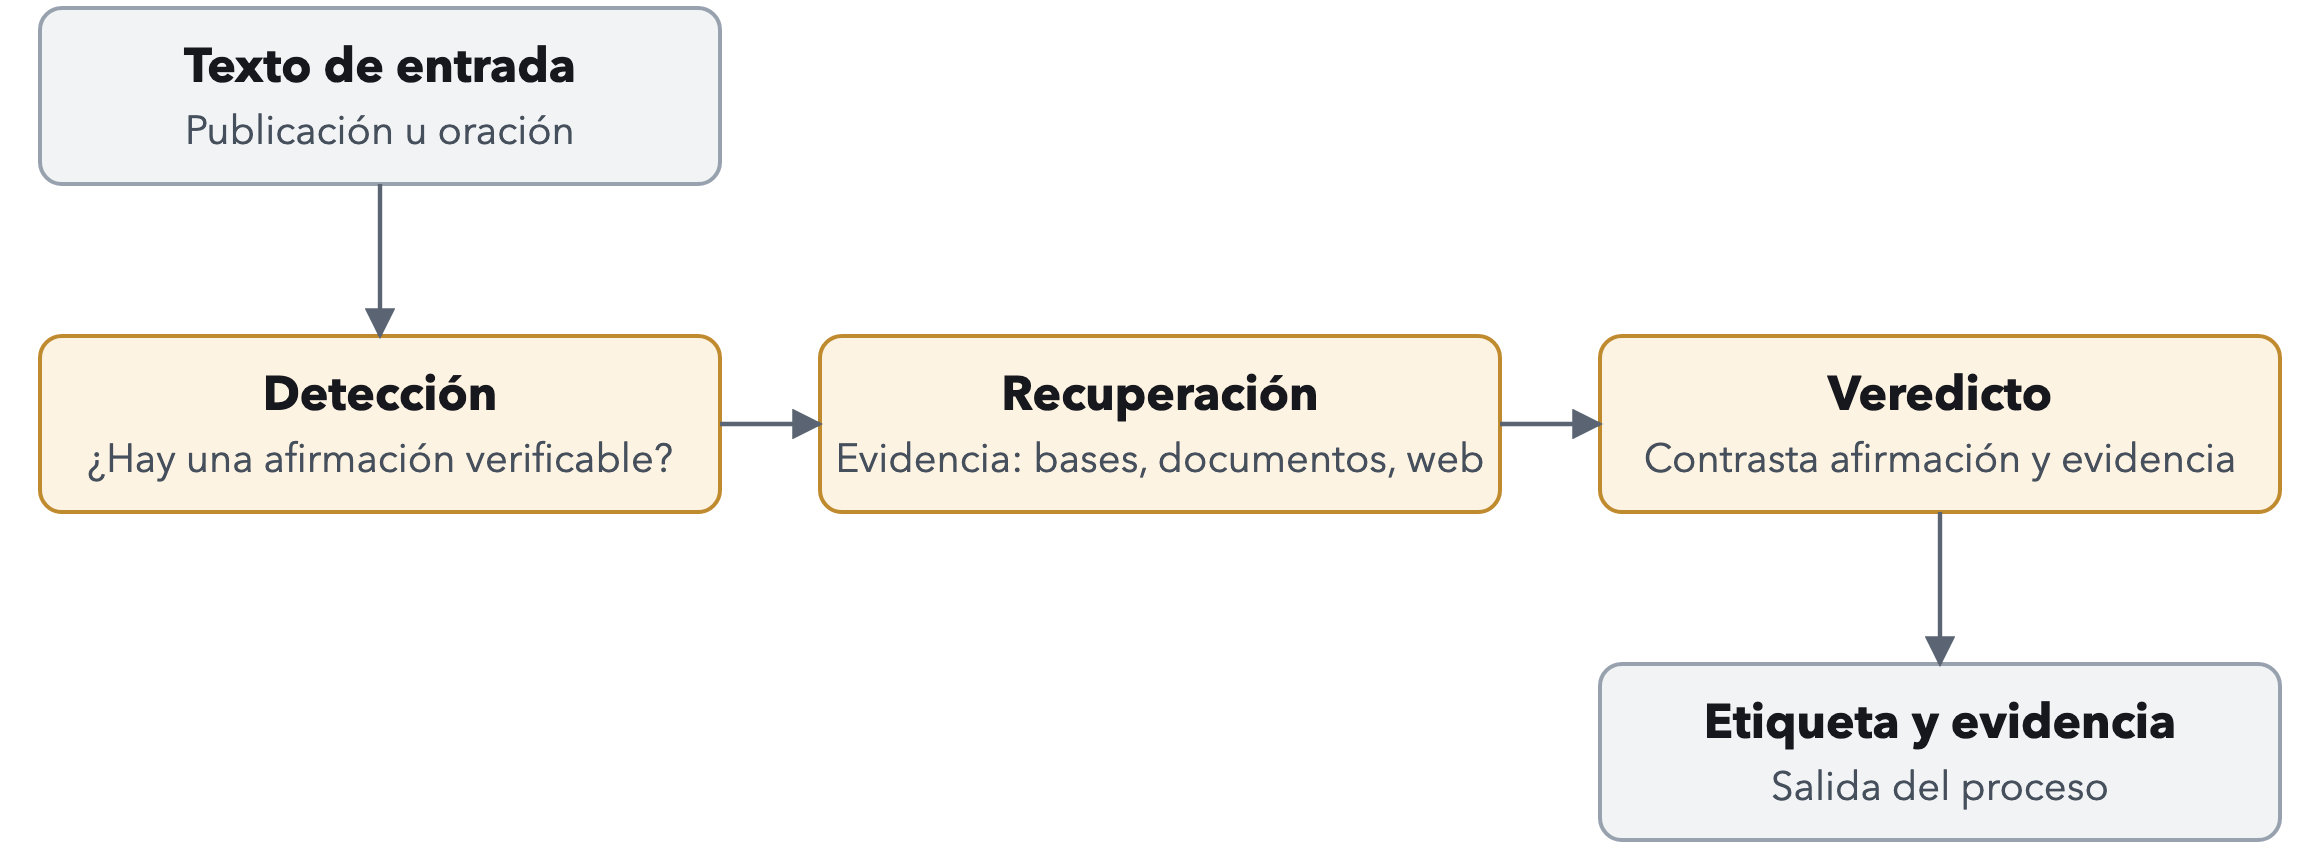
\includegraphics[width=\linewidth]{chapters/figures/pipeline}
  \caption{\textit{Pipeline} canónico de verificación automática de afirmaciones en tres etapas. Fuente: elaboración propia a partir de \textcite{GuoEtAl2022}.}
  \label{fig:pipeline}
\end{figure}

La primera etapa consiste en la identificación de afirmaciones verificables (\textit{claim detection}). No toda oración expresa una afirmación factual: las preguntas, opiniones, expresiones emocionales y declaraciones hipotéticas quedan excluidas del proceso. \textcite{PanchendrarajanZubiaga2024} sintetizan los métodos disponibles para esta tarea, que van desde clasificadores apoyados en características léxicas y sintácticas hasta arquitecturas Transformer, y señalan a estas últimas como las de mejor desempeño en los trabajos relevados.

La segunda etapa recupera evidencia externa para contrastar la afirmación identificada. Las fuentes de evidencia se agrupan en tres categorías con distintos compromisos entre cobertura y latencia. Las bases de conocimiento estructuradas, como Wikidata o Wikipedia, ofrecen un acceso eficiente pero una cobertura limitada; los corpus de documentos no estructurados, como los artículos periodísticos, amplían la cobertura a costa de una recuperación más compleja. La tercera categoría es la búsqueda web en tiempo real, que ofrece la máxima cobertura y la evidencia más actualizada a costa de una latencia superior. \textcite{TianEtAl2024} implementaron agentes de recuperación web que integran búsqueda con razonamiento mediante LLM, y reportan una mejora de hasta veinte puntos porcentuales en F1 macro respecto de los mismos modelos operando sin búsqueda.

La generación aumentada por recuperación (\textit{Retrieval-Augmented Generation}, RAG) formaliza esa combinación entre recuperación y generación. \textcite{LewisEtAl2020} la definen como un modelo generativo cuya memoria paramétrica, el conocimiento almacenado en los pesos, se complementa con una memoria no paramétrica: un índice vectorial de documentos consultado mediante un recuperador denso, cuyos pasajes se incorporan a la entrada del generador para condicionar su respuesta. Frente a un modelo que responde solo con lo aprendido durante el entrenamiento, el esquema produce texto más específico y factual, permite actualizar el conocimiento reemplazando el índice sin reentrenar y vuelve posible exhibir la procedencia de cada respuesta \parencite{LewisEtAl2020}. Esta última propiedad, el anclaje de la salida en documentos identificables (\textit{grounding}), es la que habilita la atribución: cada afirmación generada puede acompañarse del enlace al pasaje que la sustenta, de manera que el lector la contraste por su cuenta. El anclaje no garantiza por sí mismo la fidelidad, dado que el generador puede apartarse de la evidencia recuperada, y la calidad del resultado queda acotada por la del recuperador.

La tercera etapa combina la representación de la afirmación con la evidencia recuperada para producir un veredicto de veracidad. Los esquemas de etiquetado varían entre dos clases, verdadero y falso, y seis niveles de gradación, como en el \textit{dataset} LIAR \parencite{Wang2017}. El esquema binario es el más frecuente en la literatura por razones de comparabilidad con \textit{benchmarks} establecidos, aunque la clasificación de mayor granularidad captura mejor la complejidad del fenómeno real.

Cuando la evidencia es textual, el contraste entre afirmación y evidencia se modela como una tarea de detección de postura (\textit{stance detection}): dado un par formado por una afirmación y un documento, se determina si el documento la respalda, la contradice o no se pronuncia sobre ella. El \textit{Fake News Challenge} (FNC-1) planteó la tarea entre el titular y el cuerpo de una noticia, con cuatro clases: de acuerdo, en desacuerdo, discute y no relacionado. El análisis retrospectivo de \textcite{HanselowskiEtAl2018} mostró que la métrica oficial de la competencia favorecía a las clases mayoritarias y que los sistemas mejor ubicados apenas reconocían las minoritarias, en particular la de desacuerdo, que es la más informativa para la verificación; por esa razón los autores propusieron evaluarla con el valor F1 macro. FEVER \parencite{ThorneEtAl2018} trasladó la formulación a la verificación de afirmaciones: reúne 185.445 afirmaciones generadas a partir de Wikipedia, clasificadas como respaldadas (\textit{Supported}), refutadas (\textit{Refuted}) o sin información suficiente (\textit{NotEnoughInfo}), y exige recuperar, junto con la etiqueta, las oraciones que sirven de evidencia. La tercera clase de FEVER ubica la falta de evidencia en la relación entre la afirmación y los documentos disponibles, y no en el texto de la afirmación aislada.

\subsection{Redes sociales como vector de desinformación}

Las redes sociales son el canal de mayor escala de difusión de desinformación. El estudio empírico de referencia sobre esta dinámica fue realizado por \textcite{VosoughiEtAl2018}, quienes analizaron unas 126.000 cascadas de rumores verificados que circularon en X entre 2006 y 2017, difundidas por unos tres millones de personas. Los resultados muestran que la verdad tarda unas seis veces más que la falsedad en llegar a 1.500 personas y unas veinte veces más en alcanzar una profundidad de cascada de diez retransmisiones, y que las afirmaciones falsas presentan un setenta por ciento más de probabilidad de ser retransmitidas. Un hallazgo relevante es que la amplificación la producen sobre todo las personas, y no los sistemas automatizados: la mayor novedad semántica del contenido falso activa respuestas emocionales que favorecen el acto de compartir \parencite{VosoughiEtAl2018}.

El contexto argentino presenta particularidades propias. La elevada penetración de servicios de mensajería instantánea, con WhatsApp entre las plataformas más usadas para informarse \parencite{Newman2024}, introduce desinformación en entornos cerrados y cifrados de extremo a extremo, no accesibles mediante interfaces de programación públicas. Adicionalmente, el ecosistema mediático local se caracteriza por una fuerte polarización entre distintos medios de comunicación, que se reproduce en la conversación en redes sociales en comunidades separadas que comparten selectivamente el contenido afín a sus creencias, y que genera condiciones favorables para la circulación y la amplificación de contenido engañoso \parencite{CalvoAruguete2020}.

La experiencia reciente ilustra la magnitud del fenómeno en el país. La pandemia de COVID-19 estuvo acompañada de una circulación masiva de información falsa sobre tratamientos y vacunas, situación que la Organización Mundial de la Salud denominó infodemia \parencite{Zarocostas2020}, mientras que los ciclos electorales concentran la producción de contenido engañoso sobre temas económicos y político-institucionales. Estas particularidades lingüísticas y temáticas limitan la transferencia directa de modelos entrenados sobre otras lenguas y culturas.

\subsection{Métricas de evaluación}

La evaluación de los sistemas de detección de desinformación se apoya en métricas estándar de clasificación, derivadas de la matriz de confusión que contabiliza verdaderos positivos, verdaderos negativos, falsos positivos y falsos negativos. La exactitud (\textit{accuracy}) mide la proporción de predicciones correctas sobre el total, pero engaña en conjuntos de datos desbalanceados, situación habitual en este dominio donde las publicaciones verídicas suelen superar ampliamente a las falsas \parencite{GuoEtAl2022}. Por ese motivo, la literatura prioriza métricas sensibles a la distribución de clases.

La precisión cuantifica la fracción de contenidos señalados como desinformación que efectivamente lo son, mientras que la cobertura (\textit{recall}) mide la fracción de desinformación real que el sistema logra identificar. Ambas métricas se encuentran en tensión: un sistema que clasifica como falso casi todo el contenido alcanza una cobertura alta a costa de una precisión baja, con el consecuente exceso de falsos positivos. El valor F1, definido como la media armónica entre precisión y cobertura, sintetiza este compromiso en un único indicador y es la métrica de referencia más extendida en la disciplina. Formalmente, a partir de los verdaderos positivos (VP), verdaderos negativos (VN), falsos positivos (FP) y falsos negativos (FN), estas métricas se definen según las Ecuaciones~\ref{eq:precision-cobertura} y~\ref{eq:f1-exactitud}:

\begin{equation}
  \text{Precisión} = \frac{VP}{VP + FP}, \qquad
  \text{Cobertura} = \frac{VP}{VP + FN},
  \label{eq:precision-cobertura}
\end{equation}

\begin{equation}
  F_1 = 2 \cdot \frac{\text{Precisión} \cdot \text{Cobertura}}{\text{Precisión} + \text{Cobertura}}, \qquad
  \text{Exactitud} = \frac{VP + VN}{VP + VN + FP + FN}.
  \label{eq:f1-exactitud}
\end{equation}

Para evaluar el desempeño con independencia del umbral de decisión se emplea el área bajo la curva ROC (\textit{Area Under the ROC Curve}, AUC-ROC), que mide la capacidad del modelo de ordenar correctamente ejemplos positivos y negativos a lo largo de todos los umbrales posibles. En problemas con más de una clase de interés, las tres métricas se calculan por clase y se promedian: el promedio macro pondera a todas las clases por igual, mientras que el ponderado lo hace según su frecuencia, de modo que el primero penaliza el desempeño deficiente en la clase minoritaria.

La métrica que se prioriza depende del costo relativo de los dos errores. Cuando el más costoso es el falso negativo, como en el \textit{screening} de contenido destinado a una revisión humana posterior, se privilegia la cobertura. Cuando lo es el falso positivo, que en este dominio equivale a señalar como desinformación un contenido verídico, se privilegian la precisión y el control de la tasa de falsos positivos. La elección corresponde, por lo tanto, al diseño de cada sistema y no a una propiedad de la métrica.

\subsection{Combinación de señales y calibración}
\label{sec:combinacion-calibracion}

Cuando un sistema dispone de varias fuentes de información sobre un mismo caso, como el texto, los metadatos del emisor y la evidencia externa, debe integrarlas en una decisión única. La fusión temprana concatena las representaciones de entrada y entrena un único modelo; la fusión tardía, en cambio, obtiene una salida por fuente y combina esas salidas. La regla de combinación más simple es el promedio ponderado de las salidas, con pesos fijados por criterio experto o ajustados sobre datos de validación. La generalización apilada (\textit{stacking}) de \textcite{Wolpert1992} reemplaza esos pesos por un segundo nivel de aprendizaje: un metaclasificador se entrena sobre las predicciones que los modelos de base producen para ejemplos que no vieron durante su ajuste, y aprende de ellas cómo combinarlas. A cambio, el apilamiento requiere ejemplos etiquetados adicionales de los que el promedio ponderado prescinde.

Combinar salidas de modelos distintos presupone, además, que resulten comparables, y en este punto interviene la calibración. Un clasificador está calibrado cuando, entre todos los casos a los que asigna un valor $p$, la proporción de positivos es efectivamente $p$; solo en ese caso su salida admite la lectura de probabilidad. La salida de una función sigmoide o \textit{softmax} se ubica en el intervalo $[0,1]$, pero esa forma no la convierte en una probabilidad calibrada. \textcite{GuoEtAl2017} mostraron que las redes neuronales profundas actuales, a diferencia de las de una década atrás, están mal calibradas y tienden a la sobreconfianza: asignan valores cercanos a uno a predicciones que aciertan con una frecuencia sensiblemente menor. La calibración se corrige \textit{a posteriori} mediante una transformación monótona ajustada sobre un conjunto de validación. El escalado de \textcite{Platt1999}, propuesto para convertir la salida de una máquina de soporte vectorial en una probabilidad, ajusta una sigmoide sobre esa salida, y su variante de un solo parámetro, el escalado de temperatura, resultó la más eficaz para las redes neuronales en la comparación de \textcite{GuoEtAl2017}. Como la transformación es monótona, la calibración no altera el orden de los casos ni, por lo tanto, el área bajo la curva ROC. Mientras no se calibre, la salida de un clasificador, o el promedio de varias salidas, es un puntaje que ordena los casos según el grado de sospecha, pero no una probabilidad.

\subsection{Conjuntos de datos para la detección de desinformación}

El entrenamiento y la evaluación de los modelos de detección dependen de la disponibilidad de conjuntos de datos (\textit{datasets}) etiquetados. La mayoría de los recursos de referencia se construyeron en inglés y a partir de organizaciones de verificación estadounidenses, lo que condiciona tanto el idioma como las temáticas representadas. El \textit{dataset} LIAR \parencite{Wang2017} reúne 12.836 afirmaciones extraídas de PolitiFact, etiquetadas en seis niveles de veracidad, y se emplea como \textit{benchmark} para la comparación de modelos. FakeNewsNet \parencite{ShuEtAl2020} integra contenido noticioso, contexto social y datos de propagación, lo que habilita los enfoques basados en grafos. Fakeddit \parencite{NakamuraEtAl2020} aporta escala, más de un millón de publicaciones de Reddit, y carácter multimodal mediante supervisión distante.

El panorama en español es marcadamente más limitado. El \textit{Spanish Fake News Corpus} \parencite{PosadasEtAl2019}, el recurso de referencia para la lengua, contiene apenas 1.543 noticias provenientes de México y España, entre su versión original y la partición de prueba de FakeDeS 2021 \parencite{GomezAdornoEtAl2021}, una escala más de un orden de magnitud inferior a la de los corpus en inglés. La Tabla~\ref{tab:datasets} sintetiza las características de los principales conjuntos de datos disponibles y evidencia la brecha de recursos entre ambas lenguas.

\begin{table}[t]
  \centering
  \caption{Comparación de los principales conjuntos de datos para detección de desinformación. Fuente: elaboración propia a partir de \textcite{Wang2017}, \textcite{ShuEtAl2020}, \textcite{NakamuraEtAl2020}, \textcite{PosadasEtAl2019} y \textcite{GomezAdornoEtAl2021}.}
  \label{tab:datasets}
  \begin{tabular}{l c c c c c}
    \hline
    \textbf{\textit{Dataset}} & \textbf{Idioma} & \textbf{Tamaño} & \textbf{Clases} & \textbf{Contexto social} & \textbf{Multimodal} \\
    \hline
    LIAR & Inglés & 12.836 & 6 & No & No \\
    FakeNewsNet & Inglés & $\sim$23.000 & 2 & Sí & Sí \\
    Fakeddit & Inglés & 1.063.106 & 2/3/6 & Sí & Sí \\
    \textit{Spanish Fake News} & Español & 1.543 & 2 & No & No \\
    \hline
  \end{tabular}
\end{table}

\subsection{Marco normativo}
\label{sec:marco-normativo}

Un sistema de detección que opera sobre publicaciones de redes sociales recolecta datos de personas identificables, conserva documentos de terceros como evidencia, emite un juicio sobre contenido publicado y opera dentro de una red social de terceros. Cada una de esas operaciones se encuentra alcanzada por una norma distinta. A continuación se presentan las normas vigentes en la República Argentina que las regulan y las condiciones contractuales que fijan la red social sobre la que opera la extensión y la plataforma a través de la cual podría distribuirse. Su aplicación al diseño se analiza en la Sección~\ref{sec:legal}.

La Ley 25.326 de Protección de los Datos Personales regula el tratamiento de datos asentados en archivos, registros o bancos de datos, públicos o privados \parencite{CongresoNacion2000}. Define como dato personal la información de cualquier tipo referida a personas físicas o de existencia ideal determinadas o determinables (artículo 2) y exige que los datos sean ciertos, adecuados, pertinentes y no excesivos en relación con la finalidad para la que se obtuvieron, y que se destruyan cuando dejen de ser necesarios para ella (artículo 4). El tratamiento requiere el consentimiento libre, expreso e informado del titular, salvo en los supuestos que enumera el artículo 5, entre ellos el de los datos obtenidos de fuentes de acceso público irrestricto. La cesión a terceros exige, además, interés legítimo y consentimiento, que no es necesario cuando se aplica un procedimiento de disociación que vuelve inidentificables a los titulares (artículo 11). Los titulares conservan los derechos de acceso, rectificación y supresión (artículos 14 y 16). El Decreto 1558/2001 reglamenta la ley y precisa, entre otros aspectos, el ejercicio de esos derechos \parencite{PoderEjecutivoNacional2001}.

La misma ley fija tres límites adicionales. En primer lugar, califica como datos sensibles a los que revelan opiniones políticas, entre otras categorías (artículo 2), y prohíbe la formación de archivos que almacenen información que directa o indirectamente los revele; solo admite su tratamiento con finalidades estadísticas o científicas cuando no puedan ser identificados sus titulares (artículo 7, incisos 2 y 3). En la misma línea, el artículo 28 excluye de la ley a las investigaciones científicas en la medida en que los datos recogidos no puedan atribuirse a una persona determinada o determinable. En segundo lugar, el artículo 12 prohíbe transferir datos personales a países que no proporcionen niveles de protección adecuados, prohibición que el artículo 12 del decreto levanta cuando el titular consintió expresamente la cesión o cuando la protección surge de cláusulas contractuales. La autoridad de control enumera los países adecuados, entre los que figuran los Estados de la Unión Europea y no los Estados Unidos \parencite{DNPDP2016}, y fija cláusulas contractuales tipo para las transferencias hacia los demás \parencite{DNPDP2016}. En tercer lugar, la formación de archivos de datos es lícita cuando se encuentran inscriptos (artículo 3), y los particulares que formen archivos que no sean para un uso exclusivamente personal deben registrarlos ante el organismo de control (artículos 21 y 24).

La Ley 11.723 de Régimen Legal de la Propiedad Intelectual protege las obras científicas, literarias y artísticas, entre las que incluye los escritos de toda naturaleza y extensión, y reconoce al autor la facultad exclusiva de publicarlas y reproducirlas en cualquier forma (artículos 1 y 2) \parencite{CongresoNacion1933}. El artículo 10 admite que cualquiera publique, con fines didácticos o científicos, comentarios, críticas o notas referidas a una obra, incluyendo hasta mil palabras de ella y solo las partes del texto indispensables a ese efecto. El artículo 28 permite utilizar las noticias de interés general publicadas por la prensa, con la condición de expresar la fuente cuando se reproducen en su versión original.

El Código Penal tipifica los delitos contra el honor en el Título II de su Libro Segundo \parencite{CongresoNacion1984}. La calumnia consiste en la falsa imputación a una persona física determinada de un delito concreto y circunstanciado (artículo 109), y la injuria, en deshonrar o desacreditar de forma intencional a una persona física determinada (artículo 110). La redacción vigente de ambos artículos proviene de la Ley 26.551, dictada en cumplimiento de la sentencia de la Corte Interamericana de Derechos Humanos en el caso Kimel, que reemplazó la pena de prisión por la de multa y excluyó de los dos tipos las expresiones referidas a asuntos de interés público y las que no sean asertivas \parencite{CongresoNacion2009}. El artículo 113 extiende la responsabilidad a quien publica o reproduce la imputación ajena, salvo que la atribuya en forma sustancialmente fiel a la fuente pertinente, y el inciso 2 del artículo 117 bis reprime con prisión a quien proporcione a un tercero, a sabiendas, información falsa contenida en un archivo de datos personales. La acción por calumnia o injuria es privada y solo puede ejercerla el ofendido (artículo 73). El mismo código reprime, en el artículo 153 bis, el acceso sin autorización a un sistema o dato informático de acceso restringido.

La red social fija, por su parte, condiciones contractuales propias. Los términos de servicio de X, en su versión del 9 de octubre de 2026, prohíben acceder a sus servicios por medios distintos de las interfaces publicadas y la extracción automatizada de contenido (\textit{scraping}) sin consentimiento previo y por escrito, y extienden la infracción a quien facilite o asista a otros en violarlos, incluida la distribución de productos o servicios que lo permitan \parencite{XCorp2026}. Las políticas para desarrolladores prohíben, además, inferir o almacenar la afiliación o las creencias políticas de un usuario \parencite{XCorpDesarrolladores2026}. La plataforma de distribución de extensiones agrega otras condiciones. Las políticas del programa de Chrome Web Store consideran dato de usuario al contenido de los sitios con los que la persona interactúa, y exigen a toda extensión que lo trate publicar una política de privacidad, limitar su uso a la finalidad única declarada y, antes de la instalación, informar de forma destacada qué datos recolecta y obtener el consentimiento del usuario \parencite{Google2026}.

\section{Estado del arte}
\label{sec:estado-arte}

En esta sección se revisan los trabajos publicados sobre detección automática de desinformación, agrupados según la señal que explotan. En primer lugar se presentan los enfoques basados en el contenido textual, que constituyen la línea dominante. A continuación se revisan los enfoques basados en propagación, los multimodales y la detección de texto generado por modelos de lenguaje. Luego se examina la cobertura del español y del contexto argentino y se analiza la competencia, y finalmente una conclusión resume los hallazgos y la oportunidad que de ellos se desprende.

\subsection{Enfoques basados en contenido}

Los enfoques basados en el análisis del contenido textual son la línea de investigación dominante en detección de desinformación. Los métodos clásicos utilizan representaciones de bolsa de palabras con ponderación TF-IDF combinadas con clasificadores como máquinas de soporte vectorial o regresión logística. Si bien estos métodos ofrecen interpretabilidad y eficiencia computacional, sus resultados son inferiores a los de los enfoques basados en representaciones contextuales; el análisis de \textcite{Wang2017} sobre el \textit{dataset} LIAR documenta una exactitud de referencia de alrededor del 27\% para los métodos clásicos con clasificación en seis niveles de veracidad.

La adopción generalizada de la arquitectura BERT transformó el estado del arte en detección de desinformación. \textcite{KaliyarEtAl2021} propusieron FakeBERT, que combina las representaciones contextuales de BERT con capas de redes neuronales convolucionales (\textit{Convolutional Neural Networks}, CNN) para capturar patrones locales característicos del lenguaje desinformativo. El sistema alcanza resultados superiores al 98\% de exactitud bajo evaluación en el mismo dominio de entrenamiento en inglés; sin embargo, evaluaciones posteriores con datos reales revelan limitaciones de generalización. \textcite{BlancoFernandezEtAl2024} documentan una caída de entre veintiséis y veintisiete puntos porcentuales al trasladar modelos \textit{fine-tuned} del entorno de evaluación controlada a datos del mundo real en español. El fenómeno, conocido como desplazamiento de dominio, afecta de manera pronunciada a los sistemas entrenados sobre corpus en inglés y aplicados a textos en otras lenguas. La magnitud de los resultados en condiciones controladas debe interpretarse con cautela, ya que suele responder a particiones binarias y a conjuntos de prueba del mismo dominio de entrenamiento, lo que sobrestima el desempeño esperable en operación real.

La irrupción de los LLM abrió una línea de investigación que propone la detección mediante razonamiento en modo \textit{zero-shot} o \textit{few-shot}, sin entrenamiento específico. \textcite{RazaEtAl2024} compararon modelos de la familia BERT con LLM sobre un corpus de diez mil artículos anotados con asistencia de GPT-4 y verificados por personas, además de un subconjunto de NELA-GT-2022. Los modelos con \textit{fine-tuning} superan de manera consistente a los LLM operando sin ejemplos o con pocos ejemplos, mientras que estos últimos exhiben mayor robustez frente a perturbaciones del texto.

Por su parte, la revisión de \textcite{SrbaEtAl2025}, que abarca 175 publicaciones sobre evaluación automática de credibilidad textual, concluye que los LLM aportan mayor valor en tareas de generación (síntesis de evidencia, producción de explicaciones) que en clasificación directa, y recomienda arquitecturas híbridas que combinen un clasificador \textit{fine-tuned} con un LLM para la etapa de interpretación. Entre las señales textuales de credibilidad que esta línea identifica como más discriminativas se cuentan la presencia o ausencia de fuentes citadas, el uso de lenguaje sensacionalista o de alta carga emocional, la consistencia interna del texto, la concordancia con la cobertura de otros medios sobre el mismo hecho y el historial del dominio de publicación. Estas señales pueden incorporarse como características complementarias del clasificador base o extraerse mediante un LLM en la etapa de interpretación, lo que refuerza el carácter explicable del veredicto.

En el ámbito hispanohablante, \textcite{ToapantaEtAl2024} compararon cinco modelos Transformer preentrenados en español sobre un corpus de publicaciones en X verificadas por organizaciones ecuatorianas de \textit{fact-checking}. MarIA, preentrenado sobre el corpus de la Biblioteca Nacional de España, alcanzó el 96,0\,\% de exactitud, seguido de BERTin con el 95,5\,\% y de BETO, RoBERTuito y BERTuit en torno al 93,5\,\%, como muestra la Tabla~\ref{tab:toapanta}. Son los resultados más cercanos al dominio de este trabajo: muestran que el enfoque con modelos Transformer preentrenados en español es viable en el contexto latinoamericano y que, al mismo tiempo, no hay trabajos equivalentes para Argentina.

\begin{table}[t]
  \centering
  \caption{Desempeño de modelos Transformer en español sobre publicaciones verificadas en Ecuador. Fuente: elaboración propia a partir de \textcite{ToapantaEtAl2024}.}
  \label{tab:toapanta}
  \begin{tabular}{l c c}
    \hline
    \textbf{Modelo} & \textbf{Exactitud} & \textbf{F1} \\
    \hline
    MarIA & 96,0\% & 0,960 \\
    BERTin & 95,5\% & 0,954 \\
    BETO & 93,5\% & 0,935 \\
    RoBERTuito & 93,5\% & 0,934 \\
    BERTuit & 93,4\% & 0,933 \\
    \hline
  \end{tabular}
\end{table}

La situación del español encuentra un paralelo instructivo en otras lenguas con escasa cobertura de recursos. La revisión de \textcite{AlbtoushEtAl2025} sobre detección de desinformación en árabe identifica desafíos análogos a los del español: morfología compleja, diversidad de variantes dialectales y escasez de conjuntos de datos anotados frente a la abundancia de recursos en inglés. Su hallazgo central es que los modelos Transformer adaptados, a la lengua o al dominio de aplicación, superan de manera consistente a los modelos de propósito general. Ese criterio es el que ordena la elección del presente trabajo: descarta las alternativas genéricas y admite tanto a los modelos monolingües en español como a los multilingües adaptados al registro de las redes sociales, categoría a la que pertenece XLM-T. La elección dentro de esa categoría dista de ser indiferente: \textcite{GoulievEtAl2025} comparan cinco modelos multilingües sobre un mismo corpus y obtienen exactitudes que van del 79,3\,\% al 87,1\,\%, casi ocho puntos de dispersión entre el peor y el mejor. Por eso la elección no se da por cerrada de antemano, sino que se somete a una comparación experimental en la que RoBERTuito y BETO operan como líneas de contraste, junto con TF-IDF y un clasificador lineal como línea base.

\subsection{Enfoques basados en propagación}

Una segunda línea de investigación explota el patrón de difusión de la información como señal de veracidad, como complemento o como alternativa al análisis del contenido. La motivación empírica proviene de los hallazgos de \textcite{VosoughiEtAl2018} sobre las diferencias estructurales entre cascadas de noticias falsas y verdaderas en X.

\textcite{BianEtAl2020} propusieron BiGCN (\textit{Bidirectional Graph Convolutional Networks}), que modela el árbol de difusión de una publicación como un grafo dirigido y aplica redes convolucionales de grafos en dos sentidos: de arriba hacia abajo, para capturar la estructura de propagación, y de abajo hacia arriba, para incorporar señales de corrección o refutación presentes en los hilos de respuesta. El sistema supera en aproximadamente diez puntos porcentuales a los métodos basados únicamente en texto sobre un corpus de rumores en X, lo que evidencia que los patrones de propagación contienen información diagnóstica no redundante con el contenido. La aplicabilidad práctica de estos enfoques está condicionada al acceso en tiempo real a los grafos de difusión mediante interfaces de programación de las plataformas, cuya disponibilidad se ha visto restringida significativamente desde 2023.

Más allá de BiGCN, la literatura ha explorado otras formas de modelar la estructura social de la difusión. Los métodos basados en núcleos de árbol de propagación comparan la forma de las cascadas para discriminar rumores \parencite{MaEtAl2017}; modelos que integran el contenido, la respuesta de los usuarios y las características de la fuente en una representación conjunta capturan señales temporales del proceso de difusión \parencite{RuchanskyEtAl2017}; y las aproximaciones basadas en grafos heterogéneos vinculan publicaciones, usuarios y fuentes para aprovechar el contexto social de manera inductiva \parencite{NguyenEtAl2020}. El denominador común de estos enfoques es su dependencia de datos de interacción (cadenas de retransmisión, respuestas y relaciones entre cuentas) cuyo acceso programático se redujo de forma drástica tras las restricciones impuestas por las plataformas, lo que limita su viabilidad en sistemas que operan en tiempo real. Por ese motivo, el sistema se apoya en señales de contenido y de fuente, y no en el grafo de propagación.

\subsection{Enfoques multimodales}

Los enfoques multimodales combinan el análisis del texto con otras modalidades de información, principalmente imágenes, metadatos de la fuente o características del grafo de difusión. El \textit{dataset} Fakeddit \parencite{NakamuraEtAl2020}, con más de un millón de publicaciones de Reddit etiquetadas con texto e imagen mediante supervisión distante, habilitó investigaciones en clasificación multimodal a gran escala. La combinación de modalidades puede realizarse mediante fusión temprana, concatenando las representaciones de texto e imagen antes de la clasificación, fusión tardía, agregando las predicciones de modelos independientes, o esquemas intermedios basados en atención cruzada entre modalidades, cada uno con distintos compromisos entre complejidad y capacidad de capturar interacciones entre el texto y la imagen. Los enfoques multimodales presentan mayor complejidad de implementación y mayores requisitos de datos etiquetados que los sistemas de texto solamente; la versión inicial del sistema se centra en el análisis textual y deja la información visual para una extensión futura.

\subsection{Detección de texto generado por modelos de lenguaje}

La masificación de los LLM introdujo una dimensión adicional al problema: junto a la desinformación, en la que el contenido es falso con independencia de su origen, aparece el texto generado por modelos de lenguaje, cuyo rasgo distintivo es su naturaleza sintética. Esta segunda categoría es cada vez más relevante, dado que los modelos generativos permiten producir contenido desinformativo a gran escala, con apariencia verosímil y bajo costo.

Para la detección de texto sintético, la literatura distingue tres familias de métodos. Los enfoques estadísticos analizan regularidades propias de la generación automática, como la previsibilidad de los \textit{tokens}, e incluyen técnicas que comparan la probabilidad asignada por un modelo de referencia \parencite{GehrmannEtAl2019,MitchellEtAl2023}. Los enfoques basados en clasificadores entrenan modelos supervisados para distinguir texto humano de texto sintético \parencite{ZellersEtAl2019}. Por último, las técnicas de marca de agua (\textit{watermarking}) introducen señales imperceptibles durante la generación que permiten su identificación posterior \parencite{KirchenbauerEtAl2023}. La principal limitación transversal es que la rápida evolución de los modelos generativos degrada el desempeño de los detectores estáticos, lo que obliga a una actualización continua. Aunque la versión inicial del sistema se orienta a la veracidad del contenido y no a la detección de su origen, tener en cuenta este fenómeno es pertinente para anticipar la evolución del problema.

\subsection{Cobertura del español y del contexto argentino}

La investigación sobre detección de desinformación se distribuye de manera desigual entre lenguas y regiones. \textcite{WangEtAl2024survey}, en una revisión publicada como versión preliminar sin revisión por pares, documentan que el 83\% de esa investigación se realiza en inglés, con cobertura marginal del español y prácticamente inexistente para las variedades latinoamericanas. En las fuentes revisadas para este trabajo no se identificaron publicaciones académicas sobre detección automática de desinformación centradas en el contexto argentino, ni un corpus público anotado sobre el problema; los recursos en español disponibles provienen de otros países, como se detalla a continuación.

El tamaño reducido de los corpus disponibles en español es una limitación adicional. El \textit{Spanish Fake News Corpus} \parencite{PosadasEtAl2019}, el corpus de referencia más utilizado en la literatura hispanohablante, contiene 971 noticias en su versión original, a las que la competencia FakeDeS 2021 sumó una partición de prueba de 572 \parencite{GomezAdornoEtAl2021}. Aun en conjunto, esas 1.543 muestras contrastan con los 12.836 ejemplos del \textit{dataset} LIAR \parencite{Wang2017} en inglés. Esta diferencia de escala de más de un orden de magnitud restringe las posibilidades de entrenamiento y evaluación de modelos especializados en español. Las fuentes de ese corpus corresponden además a contextos de México y España, con escasa representatividad del español rioplatense y de las temáticas políticas y económicas del contexto argentino.

La brecha de generalización entre resultados en condiciones de laboratorio y desempeño en datos reales es un desafío técnico abierto. \textcite{HasanEtAl2025}, en una versión preliminar sin revisión por pares, muestran que los mejores modelos alcanzan alrededor del 62\% de exactitud en LIAR bajo evaluación cruzada entre dominios, lo que sugiere que los modelos aprenden señales espurias del dominio de entrenamiento en lugar de indicadores generalizables de veracidad. \textcite{GoulievEtAl2025} matizan ese diagnóstico. Su evaluación sobre veinticinco lenguas, que la Tabla~\ref{tab:polytruth} resume, muestra que la penalización de los modelos multilingües no recae sobre el español, que figura entre las lenguas con recursos abundantes y alcanza valores de F1 cercanos a 0,90, sino sobre las lenguas con escasa representación en los corpus de preentrenamiento, donde la caída va de trece a veintidós puntos según el modelo. La dificultad del caso argentino no proviene, entonces, del idioma en abstracto: el español está bien cubierto por los modelos disponibles. Proviene de la variedad rioplatense, de las temáticas locales y de la ausencia de datos anotados sobre ambas, que son las tres condiciones que ningún recurso público satisface. Por su parte, \textcite{DrzchalEtAl2024} desarrollaron un \textit{pipeline} de verificación automática diseñado para aplicarse en prácticamente cualquier idioma, cuyas evaluaciones publicadas excluyen sistemáticamente el español, lo que ilustra la tendencia a omitir esta lengua incluso en sistemas con pretensión de cobertura universal.

\begin{table}[t]
  \centering
  \caption{Desempeño de modelos multilingües sobre el corpus PolyTruth, medido en F1 de la clase desinformación, según la disponibilidad de recursos de la lengua. Fuente: elaboración propia a partir de \textcite{GoulievEtAl2025}.}
  \label{tab:polytruth}
  \begin{tabular}{l c c c}
    \hline
    \textbf{Modelo} & \textbf{Lenguas con recursos} & \textbf{Lenguas sin recursos} & \textbf{Diferencia} \\
    \hline
    RemBERT   & 0,91 & 0,78 & 13 \\
    XLM-R     & 0,89 & 0,74 & 15 \\
    mT5       & 0,88 & 0,72 & 16 \\
    XLM       & 0,85 & 0,67 & 18 \\
    mBERT     & 0,83 & 0,61 & 22 \\
    \hline
  \end{tabular}
\end{table}

\subsection{Análisis de competencia}
\label{sec:competencia}

En esta sección se ubica la propuesta frente a las soluciones que hoy atienden el problema y se fundamenta la existencia de un espacio de mercado que ninguna ocupa por completo. En primer lugar se relevan las soluciones comerciales y de mercado. A continuación se aplican las herramientas de la estrategia de océano azul: el espacio diferencial, la matriz de eliminar, reducir, incrementar y crear, su diccionario de variables y la curva de valor. Luego se presenta el análisis de fortalezas, oportunidades, debilidades y amenazas, y finalmente una síntesis del análisis competitivo.

\subsubsection{Soluciones comerciales y de mercado}
\label{sec:soluciones-mercado}

Más allá de la investigación académica, existe un ecosistema de soluciones aplicadas cuyo relevamiento permite ubicar el aporte del sistema propuesto frente a la oferta vigente. En el plano de la verificación manual, Chequeado es el referente argentino: fundado en 2010 como la primera iniciativa de \textit{fact-checking} de América Latina, verifica el discurso público mediante un equipo de periodistas \parencite{Chequeado2026}. La organización desarrolla además Chequeabot, un conjunto de herramientas de inteligencia artificial que identifica frases verificables en un texto y detecta afirmaciones ya chequeadas, pensado para asistir a su propio equipo y no para el lector \parencite{Chequeabot2026}. Su rigor metodológico es alto, pero la verificación sigue siendo manual, lo que limita su cobertura e impide atender el volumen y la velocidad de la desinformación en redes sociales. Herramientas de gran escala como el \textit{Fact Check Explorer} de Google agregan verificaciones publicadas por organizaciones de todo el mundo, aunque operan como buscadores de chequeos preexistentes y no analizan contenido nuevo de forma automática \parencite{GoogleFactCheck2026}.

En el segmento comercial, plataformas como Cyabra y Blackbird.AI ofrecen detección automática de campañas de desinformación, cuentas falsas y narrativas coordinadas mediante modelos de inteligencia artificial \parencite{Cyabra2026,BlackbirdAI2026}. Estas soluciones se orientan a clientes corporativos y gubernamentales (protección de marca, seguridad nacional y análisis de operaciones de influencia), operan principalmente en inglés y se comercializan bajo esquemas de licenciamiento orientados a organizaciones, sin una capa de acceso gratuito para el usuario individual. El relevamiento de este segmento se completa con Information Tracer, que sigue la difusión de enlaces en varias plataformas y calcula indicadores de manipulación del tráfico \parencite{ChenEtAl2021}, y con Newtral FactFlow, un tablero para verificadores profesionales que detecta posible desinformación en Telegram con modelos de lenguaje \parencite{JournalismAINewtral2024}.

Dentro de la propia plataforma X operan dos mecanismos dirigidos al usuario. El primero son las Notas de la Comunidad (\textit{Community Notes}): colaboradores inscriptos redactan notas de contexto sobre publicaciones que consideran engañosas, y una nota se muestra solo cuando la califican como útil colaboradores que en sus calificaciones anteriores discreparon entre sí. Desde 2025 también pueden proponer notas redactores automáticos, aunque la decisión de mostrarlas sigue en manos de las calificaciones de las personas \parencite{XCommunityNotes2026}. El mecanismo reduce la difusión del contenido señalado: una vez adjunta la nota, las retransmisiones caen un 46,1\,\% y las marcas de aprobación un 44,1\,\% \parencite{SlaughterEtAl2025}. Su alcance, sin embargo, es acotado. En la muestra de ese estudio, apenas el 16,9\,\% de las publicaciones con una nota propuesta llegó a mostrar una nota calificada como útil, cerca de la mitad de las notas se adjuntó más de 23 horas después de la publicación y el efecto fue mayor cuanto antes se adjuntaba la nota \parencite{SlaughterEtAl2025}.

El segundo mecanismo es Grok, el asistente de inteligencia artificial integrado en X, al que los usuarios mencionan en una respuesta para pedirle que verifique una publicación. Según un estudio publicado como versión preliminar sin revisión por pares, entre febrero y septiembre de 2025 Grok y el asistente de Perplexity recibieron en X más de 1,5 millones de solicitudes de verificación en inglés \parencite{RenaultEtAl2026}. Ese trabajo encuentra que algunos modelos alcanzan un nivel de acuerdo comparable al que existe entre verificadores profesionales, y también que las decisiones de diseño del proveedor pueden degradar ese desempeño. Otras evaluaciones registran problemas de trazabilidad: en una prueba de atribución de artículos periodísticos, 154 de las 200 citas de Grok~3 conducían a páginas de error \parencite{JazwinskaChandrasekar2025}.

Fuera de la plataforma, NewsGuard ofrece una extensión de navegador que muestra, junto a los enlaces que aparecen en redes sociales y buscadores, una calificación de confiabilidad del sitio de origen. Un equipo de periodistas calificó más de 35.000 fuentes con criterios declarados como no partidarios, y cada calificación se acompaña de una ficha que detalla la evaluación \parencite{NewsGuard2026}. La calificación recae sobre el medio y no sobre la afirmación. Su cobertura se concentra en nueve mercados de América del Norte, Europa y Oceanía, entre los que no figura Argentina, y el acceso del ciudadano cuesta 8 dólares mensuales tras una prueba de dos semanas \parencite{NewsGuard2026}.

La Tabla~\ref{tab:competidores} compara las ocho soluciones relevadas y la propuesta sobre un mismo conjunto de atributos. Las soluciones dirigidas al ciudadano existen, y algunas son automáticas y gratuitas, pero ninguna de las relevadas combina una señal automática sobre cada publicación con el contraste contra fuentes argentinas enlazadas, que es el espacio que el presente trabajo busca atender.

\begin{table}[t]
  \centering
  \footnotesize
  \setlength{\tabcolsep}{3pt}
  \renewcommand{\arraystretch}{1.15}
  \caption{Matriz comparativa de las soluciones existentes y de la propuesta. Fuente: elaboración propia a partir de las fuentes citadas en la Sección~\ref{sec:soluciones-mercado}.}
  \label{tab:competidores}
  \begin{tabular}{>{\raggedright\arraybackslash}p{1.85cm} >{\raggedright\arraybackslash}p{2.05cm} >{\raggedright\arraybackslash}p{2.3cm} >{\raggedright\arraybackslash}p{2.1cm} >{\raggedright\arraybackslash}p{2.1cm} >{\raggedright\arraybackslash}p{2.15cm} >{\raggedright\arraybackslash}p{1.85cm}}
    \hline
    \textbf{Solución} & \textbf{Público objetivo} & \textbf{Automatización} & \textbf{Idioma y contexto argentino} & \textbf{Costo para el ciudadano} & \textbf{Evidencia enlazada} & \textbf{Canal} \\
    \hline
    Information Tracer & Investigadores y organizaciones & Automática & Sin soporte para español & Sin acceso individual; suscripción comercial & No: detecta manipulación, no verifica hechos & Plataforma web \\
    Newtral FactFlow & Verificadores profesionales & Automática, con modelos de lenguaje & Español, sin foco argentino & Sin acceso ciudadano & Para el verificador, no para el lector & Telegram \\
    Cyabra & Empresas y gobiernos & Automática & Principalmente inglés & Sin acceso individual; licencia empresarial & No: detecta cuentas y narrativas & Plataforma web \\
    Blackbird.AI & Empresas y gobiernos & Automática & Principalmente inglés & Sin acceso individual; licencia empresarial & No: informes de riesgo narrativo & Plataforma web \\
    Chequeado & Público general y medios & Manual & Español, con foco argentino & Gratuito & Sí, en cada nota de verificación & Sitio web y redes \\
    Notas de la Comunidad & Usuarios de X & Humana; propuestas automáticas con calificación humana & Multilingüe, sin padrón de fuentes argentinas & Gratuito & Contexto en la nota, solo si se publica & Dentro de X \\
    Grok & Usuarios de X & Automática, solo a pedido & Multilingüe, sin padrón de fuentes argentinas & Incluido en la plataforma & Irregular; citas no siempre verificables & Respuesta en el hilo de X \\
    NewsGuard & Lectores de noticias y empresas & Calificación manual de sitios; visualización automática & Nueve mercados, sin Argentina & 8 dólares por mes tras dos semanas de prueba & Ficha del sitio, no de la afirmación & Extensión de navegador \\
    \hline
    \textbf{Propuesta} & Ciudadanos y periodistas argentinos & Automática en todo el recorrido & Español rioplatense, fuentes argentinas & Gratuito: señal ilimitada y cinco análisis profundos por mes & Enlace al documento de la fuente consultada & Extensión de navegador sobre X \\
    \hline
  \end{tabular}
\end{table}

\FloatBarrier
\subsubsection{Estrategia de océano azul}
\label{sec:oceano-azul}

La aplicación del enfoque de océano azul consiste en identificar el espacio que la competencia no ocupa, en lugar de disputar el que ya se encuentra ocupado \parencite{KimMauborgne2015}. La presencia de las Notas de la Comunidad y de Grok obliga a delimitar ese espacio con precisión, porque ambos atienden al ciudadano dentro de X, sin costo, y uno de ellos lo hace de forma automática. El relevamiento de la Sección~\ref{sec:soluciones-mercado} muestra, aun así, que ninguna de las soluciones relevadas reúne de forma simultánea tres características.

La primera es la cobertura automática de cada publicación visible. La verificación periodística y las Notas de la Comunidad dependen de personas y alcanzan, por eso, una fracción de las publicaciones y llegan con horas de demora \parencite{SlaughterEtAl2025}. Grok automatiza la respuesta, pero solo la produce cuando un usuario lo invoca. La propuesta calcula una señal sobre todas las publicaciones de texto que el usuario tiene en pantalla, sin que nadie la solicite, de modo que alcanza también a las de menor difusión, que en general no reciben nota. Por eso se plantea como un complemento de las Notas de la Comunidad y no como su reemplazo: la nota aporta un juicio humano consensuado sobre las publicaciones que más circulan, y la propuesta, una señal inmediata sobre el resto.

La segunda es el contraste contra fuentes confiables identificadas. Las respuestas de Grok no garantizan una fuente verificable, dado que las evaluaciones disponibles registran citas que conducen a páginas inexistentes \parencite{JazwinskaChandrasekar2025}, y el juicio queda atribuido al asistente de la propia plataforma. NewsGuard se apoya en un criterio explícito, pero califica al medio y no a la afirmación \parencite{NewsGuard2026}. La propuesta contrasta la afirmación contra los medios socios de ADEPA y las fuentes oficiales argentinas, enlaza el documento consultado y atribuye el juicio a esas fuentes, nunca al autor de la publicación.

La tercera es la adaptación al contexto local con acceso gratuito. Las plataformas comerciales se ofrecen bajo licencias orientadas a organizaciones y operan principalmente en inglés; NewsGuard cobra una suscripción al ciudadano y no cubre el mercado argentino; los mecanismos de X son gratuitos, pero operan de forma genérica, sin un padrón de fuentes locales; y la alternativa con foco argentino, Chequeado, es manual. La propuesta ofrece la señal sin límite y cinco análisis profundos por mes sin costo, con evidencia de fuentes argentinas. Cada una de las tres características tiene un antecedente en alguna de las soluciones relevadas; lo que no se registra es su combinación.

De esa observación se desprende la conclusión que orienta el resto del trabajo: la ventaja competitiva de la propuesta no reside en la técnica empleada. Los modelos de lenguaje basados en la arquitectura Transformer son tecnología ampliamente disponible, y su empleo no distingue a una solución de otra. La ventaja reside en el modelo de negocio, dado que la capa gratuita dirigida al ciudadano genera información sobre la circulación real de contenido desinformativo en el país, y esa información es el activo que se comercializa.

La entrevista al perfil de especialista, cuyo análisis se desarrolla en la Sección~\ref{sec:entrevistas}, confirma esa lectura y permite precisarla. Consultado sobre por dónde atacaría el proyecto en caso de competir con él, el entrevistado descarta la vía tecnológica y responde que competiría por distribución y por confianza percibida. La ventaja de negocio se desagrega así en dos componentes operativos: el acceso a canales de distribución, que en el caso de la propuesta son la tienda de extensiones y los acuerdos con medios y organizaciones, y la construcción de una reputación de imparcialidad, que el \textit{User Research} del Capítulo~\ref{ch:descripcion} identifica como la condición de aceptación del segmento.

\paragraph{Matriz de eliminar, reducir, incrementar y crear}

La matriz ERIC traduce el espacio diferencial en decisiones concretas sobre los atributos del producto \parencite{KimMauborgne2015}. La Figura~\ref{fig:eric} presenta su aplicación a la propuesta.

\begin{figure}[htbp]
  \centering
  \resizebox{\linewidth}{!}{%
  \begin{tikzpicture}[
      cuadro/.style={rectangle, rounded corners=6pt, draw=black!15},
      rotulo/.style={rectangle, rounded corners=9pt, text=white,
                     font=\bfseries\small, minimum height=0.62cm,
                     minimum width=3cm, anchor=north},
      item/.style={rectangle, rounded corners=4pt, draw=black!25, fill=white,
                   font=\footnotesize, text width=5.7cm, align=center,
                   minimum height=0.78cm, inner sep=3pt, anchor=north},
    ]
    % Cuadrantes
    \fill[eliminarBg, rounded corners=6pt]    (0,0)     rectangle (7,-3.75);
    \fill[reducirBg, rounded corners=6pt]     (7.4,0)   rectangle (14.4,-3.75);
    \fill[incrementarBg, rounded corners=6pt] (0,-3.95) rectangle (7,-9.1);
    \fill[crearBg, rounded corners=6pt]       (7.4,-3.95) rectangle (14.4,-9.1);

    % Rotulos
    \node[rotulo, fill=eliminarFg]    at (3.5,-0.25)  {ELIMINAR};
    \node[rotulo, fill=reducirFg]     at (10.9,-0.25) {REDUCIR};
    \node[rotulo, fill=incrementarFg] at (3.5,-4.2)   {INCREMENTAR};
    \node[rotulo, fill=crearFg]       at (10.9,-4.2)  {CREAR};

    % Eliminar
    \node[item] at (3.5,-1.15) {Análisis de propagación mediante grafos};
    \node[item] at (3.5,-2.15) {Detección de cuentas automatizadas};

    % Reducir
    \node[item] at (10.9,-1.15) {Multimodalidad: imagen, video y audio};
    \node[item] at (10.9,-2.15) {Verificación manual};
    \node[item] at (10.9,-3.15) {Cobertura multilingüe};

    % Incrementar
    \node[item] at (3.5,-5.1) {Automatización del proceso};
    \node[item] at (3.5,-6.1) {Velocidad de respuesta};
    \node[item] at (3.5,-7.1) {Accesibilidad para el ciudadano};
    \node[item] at (3.5,-8.1) {Evidencia verificable};

    % Crear
    \node[item] at (10.9,-5.1) {Información sobre circulación local};
    \node[item] at (10.9,-6.1) {Señal sobre cada publicación visible};

    % Nucleo
    \node[circle, fill=black!72, text=white, font=\bfseries,
          minimum size=1.5cm] at (7.2,-3.85) {ERIC};
  \end{tikzpicture}}
  \caption{Matriz de eliminar, reducir, incrementar y crear aplicada a la propuesta. Fuente: elaboración propia.}
  \label{fig:eric}
\end{figure}

\paragraph{Diccionario de variables}

Las once variables que integran la matriz requieren una definición operativa que precise qué comprende cada una, dado que el nombre del atributo no basta para determinar su alcance. La definición se enuncia a continuación encabezada por el verbo de la acción correspondiente.

\subparagraph{Eliminar}
\begin{itemize}[leftmargin=1.1cm, topsep=2pt, itemsep=2pt]
  \item \textit{Análisis de propagación mediante grafos}: eliminar el modelado de la red de difusión, es decir, qué cuenta retransmitió a qué otra y en qué orden, que requiere datos de la API de la plataforma y aporta complejidad sin retorno proporcional en un prototipo.
  \item \textit{Detección de cuentas automatizadas}: eliminar el juicio sobre la naturaleza humana o automatizada de la cuenta emisora, dado que el objeto de análisis es el contenido.
\end{itemize}

\subparagraph{Reducir}
\begin{itemize}[leftmargin=1.1cm, topsep=2pt, itemsep=2pt]
  \item \textit{Multimodalidad}: acotar el análisis al texto, difiriendo el tratamiento de imagen, video y audio a versiones posteriores del producto.
  \item \textit{Verificación manual}: reducir a cero la intervención humana en la producción del veredicto, dado que automatizarla es el objeto del trabajo.
  \item \textit{Cobertura multilingüe}: acotar el dominio de datos y de evidencia al español rioplatense, aun cuando el modelo subyacente procese varias lenguas.
\end{itemize}

\subparagraph{Incrementar}
\begin{itemize}[leftmargin=1.1cm, topsep=2pt, itemsep=2pt]
  \item \textit{Automatización del proceso}: extender la ejecución automática a la totalidad del recorrido, desde la lectura de la publicación hasta la presentación del veredicto.
  \item \textit{Velocidad de respuesta}: reducir de horas o días a segundos el tiempo que transcurre hasta la obtención del veredicto, intervalo que determina si la advertencia llega antes o después de que el contenido circuló.
  \item \textit{Accesibilidad para el ciudadano}: ampliar el acceso a cualquier persona que disponga de un navegador, sin costo y sin conocimiento técnico previo: la señal automática no tiene límite de uso y la versión gratuita incluye cinco análisis profundos por mes.
  \item \textit{Evidencia verificable}: aumentar aquello que el usuario puede comprobar por sus propios medios, mediante los enlaces a las fuentes consultadas y el desglose de los puntajes parciales.
\end{itemize}

\subparagraph{Crear}
\begin{itemize}[leftmargin=1.1cm, topsep=2pt, itemsep=2pt]
  \item \textit{Información sobre circulación local}: crear un registro de qué contenido desinformativo circula en Argentina, en qué volumen y sobre qué temas, que ningún actor produce en la actualidad y que es el activo comercial de la propuesta.
  \item \textit{Señal sobre cada publicación visible}: crear una indicación automática, calculada sin que el usuario la solicite, sobre todas las publicaciones de texto que aparecen en pantalla, que señala cuáles conviene revisar antes de pedir el análisis profundo y alcanza a las publicaciones de menor difusión, que en general no reciben verificación.
\end{itemize}

\paragraph{Curva de valor}

La curva de valor compara el nivel de oferta de la propuesta frente al de sus competidores sobre las variables definidas \parencite{KimMauborgne2015}. Su construcción exige traducir a una escala común los atributos que la Tabla~\ref{tab:competidores} describe de forma cualitativa. Se adoptó una escala de seis niveles, de 0 a 5, donde 0 indica que la capacidad se encuentra ausente, 1 que es marginal o incidental, 2 que está presente con limitaciones significativas, 3 que está presente, 4 que es una fortaleza declarada del producto y 5 que se cuenta entre sus capacidades centrales. La asignación se realizó a partir de la documentación pública de cada competidor y de las evaluaciones independientes citadas en la Sección~\ref{sec:soluciones-mercado}.

La curva incluye solo las soluciones dirigidas al ciudadano: Chequeado, las Notas de la Comunidad, Grok y NewsGuard. Cyabra, Blackbird.AI, Information Tracer y Newtral FactFlow se omiten porque no ofrecen acceso al ciudadano y, por lo tanto, no compiten por el mismo usuario; su posicionamiento figura en la Tabla~\ref{tab:competidores}.

Los puntajes de las tres soluciones distintas de Chequeado se fundamentan en esas fuentes. Las Notas de la Comunidad obtienen 5 en verificación manual y en accesibilidad, porque el juicio humano es el núcleo del mecanismo y la nota se muestra a todo usuario de X sin instalar nada. Obtienen 2 en automatización, porque los redactores automáticos proponen notas pero no deciden su publicación, y 1 en velocidad y en señal sobre cada publicación, dado que solo una minoría de las publicaciones con nota propuesta llega a mostrarla, con horas de demora \parencite{XCommunityNotes2026,SlaughterEtAl2025}. Grok obtiene 5 en automatización y 4 en velocidad, porque responde en el hilo sin intervención humana; 4 en accesibilidad, porque requiere que el usuario lo invoque de forma pública; 2 en evidencia verificable, por la irregularidad de sus citas; y 1 en señal sobre cada publicación, porque solo actúa a pedido \parencite{RenaultEtAl2026,JazwinskaChandrasekar2025}. NewsGuard obtiene 5 en verificación manual, porque sus calificaciones las elaboran periodistas; 3 en evidencia verificable, porque la ficha detalla la evaluación del medio pero no la de la afirmación; 2 en accesibilidad, por la suscripción paga; y 2 en señal sobre cada publicación, porque muestra su calificación junto a cada enlace a un sitio calificado, aunque no evalúa el contenido \parencite{NewsGuard2026}.

En las cinco variables provenientes de las acciones de eliminar y reducir, un valor menor representa una ventaja para la propuesta, dado que corresponden a capacidades que se decidió deliberadamente no construir. Esas variables se señalan con un asterisco en la Figura~\ref{fig:curva-valor}.

\begin{landscape}
\begin{figure}[p]
  \centering
  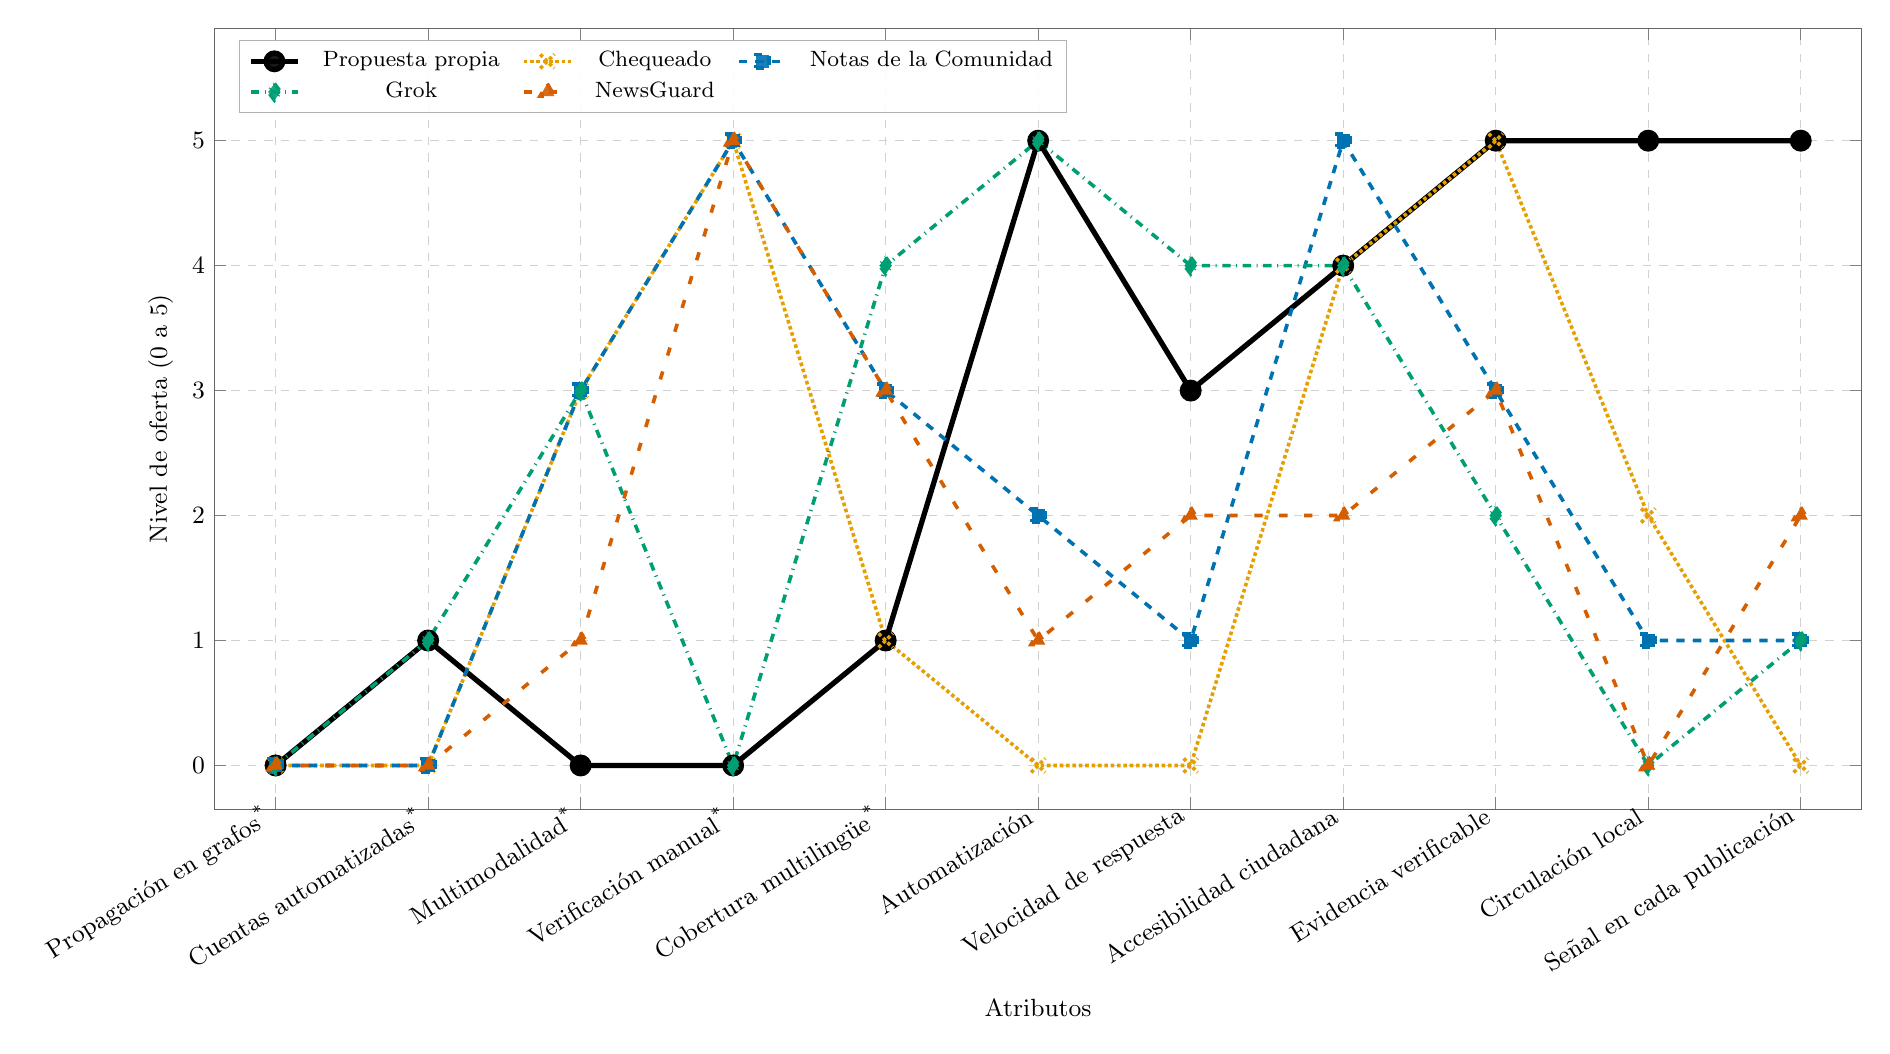
\begin{tikzpicture}
    \begin{axis}[
      width=22.5cm, height=11.5cm,
      ymin=-0.35, ymax=5.9,
      ytick={0,1,2,3,4,5},
      ylabel={Nivel de oferta (0 a 5)},
      xlabel={Atributos},
      xmin=0.6, xmax=11.4,
      xtick={1,2,3,4,5,6,7,8,9,10,11},
      xticklabels={%
        {Propagación en grafos\textsuperscript{*}},
        {Cuentas automatizadas\textsuperscript{*}},
        {Multimodalidad\textsuperscript{*}},
        {Verificación manual\textsuperscript{*}},
        {Cobertura multilingüe\textsuperscript{*}},
        {Automatización},
        {Velocidad de respuesta},
        {Accesibilidad ciudadana},
        {Evidencia verificable},
        {Circulación local},
        {Señal en cada publicación}},
      x tick label style={rotate=32, anchor=east, font=\small},
      y tick label style={font=\small},
      label style={font=\small},
      legend style={at={(0.015,0.985)}, anchor=north west, font=\footnotesize,
                    legend columns=3, draw=black!30, fill=white, fill opacity=0.9,
                    text opacity=1, column sep=6pt},
      grid=major, grid style={dashed, black!18},
      axis line style={black!60},
      ]
      \addplot[line width=1.9pt, mark=*, mark size=3pt, color=black]
        coordinates {(1,0)(2,1)(3,0)(4,0)(5,1)(6,5)(7,3)(8,4)(9,5)(10,5)(11,5)};
      \addlegendentry{Propuesta propia}

      \addplot[densely dotted, line width=1.3pt, mark=x, mark size=3.6pt, color={rgb,255:red,230;green,159;blue,0}]
        coordinates {(1,0)(2,0)(3,3)(4,5)(5,1)(6,0)(7,0)(8,4)(9,5)(10,2)(11,0)};
      \addlegendentry{Chequeado}

      \addplot[dashed, line width=1.3pt, mark=square*, mark size=2.4pt, color={rgb,255:red,0;green,114;blue,178}]
        coordinates {(1,0)(2,0)(3,3)(4,5)(5,3)(6,2)(7,1)(8,5)(9,3)(10,1)(11,1)};
      \addlegendentry{Notas de la Comunidad}

      \addplot[dashdotted, line width=1.3pt, mark=diamond*, mark size=3pt, color={rgb,255:red,0;green,158;blue,115}]
        coordinates {(1,0)(2,1)(3,3)(4,0)(5,4)(6,5)(7,4)(8,4)(9,2)(10,0)(11,1)};
      \addlegendentry{Grok}

      \addplot[loosely dashed, line width=1.3pt, mark=triangle*, mark size=3pt, color={rgb,255:red,213;green,94;blue,0}]
        coordinates {(1,0)(2,0)(3,1)(4,5)(5,3)(6,1)(7,2)(8,2)(9,3)(10,0)(11,2)};
      \addlegendentry{NewsGuard}
    \end{axis}
  \end{tikzpicture}
  \caption{Curva de valor de la propuesta frente a las soluciones dirigidas al ciudadano. Los atributos señalados con asterisco corresponden a capacidades cuya construcción se descartó, en las que conviene un valor menor. Fuente: elaboración propia.}
  \label{fig:curva-valor}
\end{figure}
\end{landscape}

La curva evidencia que la propuesta no alcanza el nivel máximo en todas las variables, circunstancia esperable y coherente con la matriz. Obtiene el valor más bajo del conjunto, solo o compartido, en cuatro de las cinco primeras, que son precisamente aquellas cuya construcción se descartó. En cuentas automatizadas obtiene 1, por encima de Chequeado, de las Notas de la Comunidad y de NewsGuard, porque el módulo de señales de la cuenta considera rasgos públicos de la cuenta autora, aunque no se propone identificar cuentas automatizadas. En velocidad de respuesta obtiene 3, por debajo de Grok: la señal automática se estima en menos de medio segundo, pero no emite veredicto, y el análisis profundo, que sí lo emite, registró una mediana de 8,5 segundos y un percentil 95 de 16,0 segundos en la medición del prototipo descrita en la Sección~\ref{sec:mediciones-rnf}, por encima de la meta de ocho segundos. En accesibilidad obtiene 4, por debajo de las Notas de la Comunidad, que se muestran a todo usuario de X, mientras que la propuesta requiere instalar la extensión y acota el análisis profundo a cinco por mes en la versión gratuita.

El despegue respecto de las demás soluciones se produce en tres variables. En evidencia verificable, solo Chequeado iguala a la propuesta, y lo hace sin automatización. En las dos variables creadas, la distancia respecto del competidor más próximo es de tres puntos: Chequeado produce un registro parcial de la circulación local a partir de lo que decide verificar, y NewsGuard muestra su calificación junto a cada enlace, aunque sobre el sitio y no sobre el contenido. Ninguna solución dirigida al ciudadano combina una señal automática sobre cada publicación con evidencia enlazada a fuentes argentinas, y esa intersección es el espacio que la propuesta ocupa. La información sobre circulación local es, además, la variable que sostiene el modelo de negocio descrito en la Sección~\ref{sec:negocio}.

\subsubsection{Análisis de fortalezas, oportunidades, debilidades y amenazas}

La Tabla~\ref{tab:foda} presenta el análisis FODA \parencite{KotlerKeller2016} de la propuesta, que organiza los factores internos y externos según su incidencia positiva o negativa sobre la viabilidad del proyecto.

\begin{table}[t]
  \centering
  \small
  \caption{Análisis de fortalezas, oportunidades, debilidades y amenazas. Fuente: elaboración propia.}
  \label{tab:foda}
  \begin{tabular}{p{1.6cm} p{5.6cm} p{5.6cm}}
    \hline
    & \textbf{Positivo} & \textbf{Negativo} \\
    \hline
    \textbf{Interno} &
    \textbf{Fortalezas.} Conjunto de datos difícil de replicar sin adopción ciudadana. Foco en el español rioplatense y en fuentes argentinas. Evidencia verificable y no únicamente un veredicto. Costos operativos reducidos durante el desarrollo &
    \textbf{Debilidades.} El modelo depende íntegramente de lograr adopción. Riesgo de falsos positivos ante sátira e ironía. Equipo reducido. El clasificador requiere entrenamiento y validación continuos \\
    \textbf{Externo} &
    \textbf{Oportunidades.} Ciclos electorales recurrentes con alta demanda de monitoreo. La inteligencia artificial generativa como vector creciente de desinformación. Ausencia de un competidor local automático con foco ciudadano. Las Notas de la Comunidad alcanzan una fracción de las publicaciones y con demora, lo que deja lugar a un complemento automático. Tendencia regulatoria hacia la transparencia algorítmica &
    \textbf{Amenazas.} Regulación sobre el tratamiento de datos. Cambios en las plataformas que limiten la extracción de contenido. Asistentes integrados en la plataforma, como Grok, que respondan dentro de X sin instalar nada. Que las Notas de la Comunidad reduzcan su demora con redactores automáticos. Que NewsGuard u otro competidor establecido extienda su cobertura al mercado argentino. Riesgo reputacional si el producto se percibe como sesgado \\
    \hline
  \end{tabular}
\end{table}

\subsubsection{Síntesis del análisis competitivo}
\label{sec:sintesis-competencia}

El relevamiento muestra que las soluciones existentes se reparten en tres grupos. La verificación periodística, con Chequeado como referente, ofrece rigor y foco argentino, pero depende de un proceso manual que no alcanza el volumen ni la velocidad con que el contenido circula en redes sociales, y los agregadores como el \textit{Fact Check Explorer} se limitan a recuperar chequeos ya publicados. Las plataformas automáticas, como Cyabra, Blackbird.AI e Information Tracer, operan a escala y en tiempo real, aunque se dirigen a organizaciones, se comercializan mediante licencias empresariales y trabajan principalmente en inglés; Newtral FactFlow automatiza la verificación en español, pero para verificadores profesionales y sobre Telegram. El tercer grupo llega al ciudadano mientras lee: dentro de X, las Notas de la Comunidad aportan un juicio humano consensuado que alcanza a una fracción de las publicaciones y con horas de demora, y Grok responde de forma automática, pero solo a pedido y sin garantía de fuentes verificables; fuera de la plataforma, NewsGuard califica sitios y no afirmaciones, mediante una suscripción paga y sin cobertura del mercado argentino.

Frente a ese panorama, la propuesta no es la única solución automática ni la única gratuita al alcance del ciudadano. Su diferencia, en la medida en que el relevamiento permite afirmarla, reside en la combinación de una señal automática sobre cada publicación visible con el contraste contra un padrón de fuentes argentinas confiables, cuyo documento se enlaza y a las que se atribuye el juicio. Por ese motivo se plantea como complemento de las Notas de la Comunidad: estas cubren con juicio humano las publicaciones que más circulan, y la propuesta alcanza a las de menor difusión, que en general no reciben nota. La curva de valor de la Figura~\ref{fig:curva-valor} expresa esa combinación en las variables de evidencia verificable y de señal sobre cada publicación, y muestra también dónde la propuesta queda por debajo de otras soluciones, como la velocidad del análisis profundo. Para ocupar ese espacio, la propuesta renuncia de forma deliberada a capacidades que la competencia sí ofrece, como el análisis de propagación y la multimodalidad, según la matriz de la Figura~\ref{fig:eric}.

La ventaja resultante no es técnica. Los modelos basados en la arquitectura Transformer están al alcance de cualquier competidor, y el especialista entrevistado señala que la disputa se libraría por distribución y por confianza percibida. La ventaja reside en el modelo de negocio: la capa gratuita genera un registro de la circulación de desinformación en Argentina que ningún actor produce en la actualidad, y ese registro es el activo que se ofrece a organizaciones. El análisis de la Tabla~\ref{tab:foda} advierte el costo de esa apuesta, porque el modelo depende por completo de lograr adopción y de sostener una reputación de imparcialidad.

En síntesis, la propuesta evita disputar el terreno de las soluciones existentes y ocupa el segmento que estas atienden solo en parte: el ciudadano argentino que necesita saber, en el momento de leer una publicación que todavía no tiene nota, si esta tiene respaldo en fuentes verificables. El Capítulo~\ref{ch:descripcion} contrasta esa hipótesis con la evidencia del \textit{User Research} y la traduce en un modelo de negocio.

\subsection{Conclusión}
\label{sec:eda-conclusion}

El relevamiento muestra, en primer lugar, una brecha técnica. La detección basada en el contenido textual alcanza resultados elevados con modelos de la familia BERT con \textit{fine-tuning} para la tarea, también en español y en lenguas con escasos recursos \parencite{KaliyarEtAl2021,ToapantaEtAl2024,AlbtoushEtAl2025}, pero esos resultados caen de forma marcada cuando el modelo se evalúa sobre datos reales o de otro dominio \parencite{BlancoFernandezEtAl2024,HasanEtAl2025}. En la literatura revisada, los LLM aportan sobre todo en la síntesis de evidencia y en la explicación del veredicto, lo que lleva a recomendar arquitecturas híbridas \parencite{RazaEtAl2024,SrbaEtAl2025}, y la recuperación de evidencia externa mejora el desempeño de los sistemas de verificación \parencite{TianEtAl2024}. Los enfoques de propagación y multimodales aportan señales no redundantes con el texto, a costa de depender de datos de interacción cuyo acceso las plataformas restringieron \parencite{BianEtAl2020,NakamuraEtAl2020}.

En segundo lugar, la brecha es de datos y no de idioma. La investigación se concentra en inglés \parencite{WangEtAl2024survey,DrzchalEtAl2024}, aunque los modelos multilingües procesan bien el español \parencite{GoulievEtAl2025}. Lo que falta son datos anotados: el corpus de referencia en español reúne 1.543 noticias de México y España \parencite{PosadasEtAl2019,GomezAdornoEtAl2021}, y en las fuentes revisadas no se identificó un corpus público sobre el contexto argentino. Una guía de etiquetado y un procedimiento reproducible para construir conjuntos de prueba con publicaciones argentinas, a partir de verificaciones ya publicadas, responden a esa ausencia.

En tercer lugar, la oferta aplicada deja un hueco preciso. La verificación profesional y las Notas de la Comunidad son eficaces cuando llegan: una nota visible reduce las retransmisiones en torno a un 46~\%, pero solo el 16,9~\% de las publicaciones con una nota propuesta llega a mostrarla, con una demora mediana cercana a las 23 horas \parencite{SlaughterEtAl2025}. Las publicaciones de difusión moderada, que en general no reciben nota, quedan sin asistencia, y ninguna solución disponible brinda al ciudadano una verificación automática, gratuita y apoyada en fuentes argentinas enlazadas.

La relevancia del problema excede el plano técnico, porque la información falsa se difunde en las redes sociales más lejos y más rápido que la verdadera \parencite{VosoughiEtAl2018}. El aporte social que se propone apunta al hueco descrito: una señal automática sobre cada publicación visible alcanza también al contenido que no se vuelve viral, y un resultado que muestra las fuentes que respaldan o contradicen la afirmación, en lugar de un dictamen, favorece que la persona ejerza su propio juicio. El aporte no es una innovación algorítmica, sino la aplicación de tecnología disponible a un dominio que la literatura no cubre. Si la señal reduce la difusión de contenido falso es una hipótesis que este trabajo no mide, y la viabilidad del sistema depende de su capacidad de alcanzar al usuario y de resultarle confiable, cuestión que el Capítulo~\ref{ch:descripcion} contrasta con el \textit{User Research}.

